% helen_doctrine.tex — camera-ready one-pager of the locked HELEN doctrine
% Sibling to HELEN_MATH_FACE_PROTOCOL.tex (the longer formal spec).
% Use this file when you need a single-page publication-grade positioning doc.
\documentclass[10pt]{article}
\usepackage[margin=1in]{geometry}
\usepackage{amsmath,amssymb,booktabs,array}
\usepackage{microtype}
\usepackage{enumitem}
\usepackage{hyperref}
\usepackage{tikz}
\usetikzlibrary{arrows.meta,positioning,shapes.geometric}
\newcommand{\cM}{\mathcal{M}}
\newcommand{\cZ}{\mathcal{Z}}
\newcommand{\cI}{\mathcal{I}}
\newcommand{\op}{\oplus}
\title{\vspace{-1.2em}\textbf{HELEN Doctrine: Closed-Loop Identity Control for Semantic-Compressed Video Editing (SCVE)}\vspace{-0.6em}}
\author{}
\date{\vspace{-1.2em}}
\begin{document}
\maketitle
\vspace{-1.0em}
\noindent\textbf{Three canonical lines (use everywhere).}
\begin{itemize}[leftmargin=1.2em,itemsep=0.15em,topsep=0.2em]
\item \textbf{Core claim:} HELEN is a \textbf{dual-render identity compiler}: one mathematical identity, multiple renderer realizations.
\item \textbf{Emergent property:} \textbf{persistent emotional identity under cheap transformation}.
\item \textbf{Business value:} maximum artistic coherence per credit spent.
\end{itemize}
\vspace{0.35em}
\noindent\textbf{Thesis (strongest sentence).}
\begin{quote}\small
\textbf{Semantic compression of video editing:} you edit \emph{meaning} in latent space instead of paying to re-solve pixels and identity every frame.
\end{quote}
\vspace{-0.4em}
\section*{1.\;Product statement (one paragraph)}
\noindent
HELEN is a \textbf{closed-loop identity control system} for semantic-compressed video editing: a mathematically anchored character can be rendered, verified, edited, and temporally propagated across styles and emotions at minimal inference cost. The system is designed so that identity is \emph{compiled once} and then \emph{transported cheaply} via low-dimensional control updates, with retries incurred only upon gate failure.
\section*{2.\;Technical architecture (minimal correct form)}
\vspace{-0.25em}
\noindent\textbf{Factorized latent state.}
\[
z_t \;=\; z_{\mathrm{id}} \;\oplus\; z_{\mathrm{control},t} \;\oplus\; z_{\mathrm{style},t} \;\oplus\; z_{\mathrm{temporal},t}.
\]
\vspace{-0.4em}
\begin{itemize}[leftmargin=1.2em,itemsep=0.15em,topsep=0.2em]
\item $z_{\mathrm{id}}$: identity invariants (anchored).
\item $z_{\mathrm{control},t}$: acting (emotion, pose, camera intent).
\item $z_{\mathrm{style},t}$: rendering/aesthetic treatment (cross-style edits).
\item $z_{\mathrm{temporal},t}$: continuity stabilizer (optional; for video).
\end{itemize}
\noindent\textbf{Compiler path (math $\to$ latent).}
\[
m\in\cM \xrightarrow{H}\; z_{\mathrm{id}} \oplus z_{\mathrm{control},0} \oplus z_{\mathrm{style},0}\;(\oplus z_{\mathrm{temporal},0}).
\]
\noindent\textbf{Dual realization (REAL + TWIN).}
\[
I_{\text{real},t}=G_{\text{real}}(A_{\text{real}}(z_t)),
\qquad
I_{\text{twin},t}=G_{\text{twin}}(A_{\text{twin}}(z_t)).
\]
\noindent\emph{Important:} $A_{\text{real}},A_{\text{twin}}$ are \textbf{renderer adapters} (format/conditioning alignment), not identity remappers.
\section*{3.\;Verification protocol (what makes it invention-grade)}
\vspace{-0.25em}
\noindent\textbf{Modality-specific identity regions.}
``Same identity'' does \emph{not} mean ``same embedding space.'' It means each output lies in a calibrated acceptance region \emph{per modality}:
\[
d_{\text{real}}\!\left(\mathrm{Emb}_{\text{real}}(I_{\text{real},t}),\mu_{\text{real}}\right)\le \tau_{\text{real}},
\qquad
d_{\text{twin}}\!\left(\mathrm{Emb}_{\text{twin}}(I_{\text{twin},t}),\mu_{\text{twin}}\right)\le \tau_{\text{twin}}.
\]
REAL uses a photoreal face embedder (e.g.\ ArcFace). TWIN uses an anime-appropriate embedder (or CLIP-face proxy initially).
\vspace{0.25em}
\noindent\textbf{Closed loop: render $\to$ gate $\to$ (invert) $\to$ correct.}
\begin{enumerate}[leftmargin=1.6em,itemsep=0.15em,topsep=0.2em]
\item propose $z_t$ (update control/style/temporal; keep $z_{\mathrm{id}}$ anchored)
\item render (REAL, TWIN)
\item gate both outputs
\item on failure: small corrective step in latent (or retry with minimal changes)
\item optional inversion for cycle consistency (v0.5+)
\end{enumerate}
\noindent\textbf{Non-negotiable experimental principle:} all experiments must center on \texttt{clone\_from\_latent}$(z_t)$ to ensure slice isolation and scientific validity.
\section*{4.\;Cost moat (formal intuition)}
\vspace{-0.25em}
\noindent\textbf{Naive video generation:}
\[
\mathrm{cost/frame}_{\text{naive}} \approx
\text{full identity solve}+\text{full style solve}+\text{full temporal solve}.
\]
\noindent\textbf{HELEN (semantic transport):}
\[
\mathrm{cost/frame}_{\text{HELEN}} \approx
\Delta z_{\mathrm{control}} + \Delta z_{\mathrm{style}} + \Delta z_{\mathrm{temporal}}
+ \text{retry tax only on gate failure}.
\]
\noindent\emph{Why this matters:} identity is compiled once and transported cheaply; failure is detected early by gates, reducing wasted generations.
\section*{5.\;System loop diagram (tight figure)}
\vspace{-0.25em}
\begin{center}
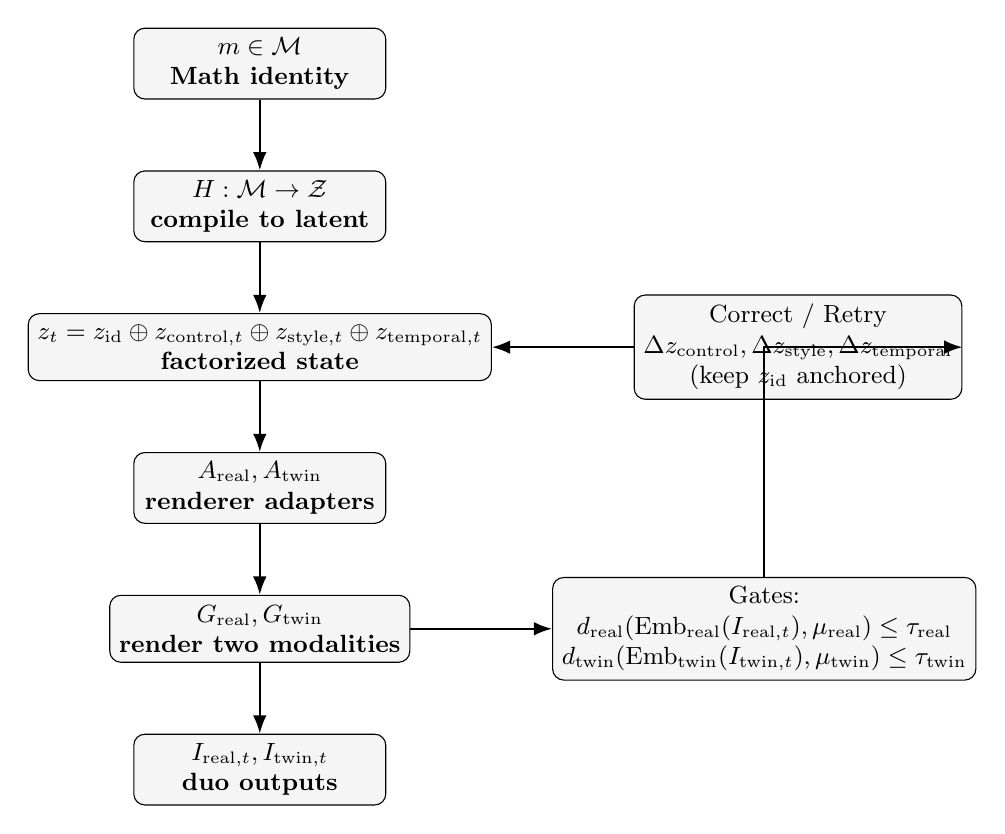
\begin{tikzpicture}[node distance=0.9cm, font=\small]
\tikzstyle{box}=[rectangle, rounded corners, draw=black, fill=gray!8, minimum height=0.85cm, minimum width=3.2cm, align=center]
\tikzstyle{arrow}=[-Latex, thick]
\node (m) [box] {$m\in\cM$\\\textbf{Math identity}};
\node (H) [box, below=of m] {$H:\cM\to\cZ$\\\textbf{compile to latent}};
\node (z) [box, below=of H] {$z_t=z_{\mathrm{id}}\oplus z_{\mathrm{control},t}\oplus z_{\mathrm{style},t}\oplus z_{\mathrm{temporal},t}$\\\textbf{factorized state}};
\node (A) [box, below=of z] {$A_{\text{real}},A_{\text{twin}}$\\\textbf{renderer adapters}};
\node (G) [box, below=of A] {$G_{\text{real}},G_{\text{twin}}$\\\textbf{render two modalities}};
\node (I) [box, below=of G] {$I_{\text{real},t}, I_{\text{twin},t}$\\\textbf{duo outputs}};
\node (gate) [box, right=1.8cm of G, minimum width=3.6cm] {Gates:\\$d_{\text{real}}(\mathrm{Emb}_{\text{real}}(I_{\text{real},t}),\mu_{\text{real}})\le\tau_{\text{real}}$\\$d_{\text{twin}}(\mathrm{Emb}_{\text{twin}}(I_{\text{twin},t}),\mu_{\text{twin}})\le\tau_{\text{twin}}$};
\node (corr) [box, right=1.8cm of z, minimum width=3.6cm] {Correct / Retry\\$\Delta z_{\mathrm{control}},\Delta z_{\mathrm{style}},\Delta z_{\mathrm{temporal}}$\\(keep $z_{\mathrm{id}}$ anchored)};
\draw[arrow] (m) -- (H);
\draw[arrow] (H) -- (z);
\draw[arrow] (z) -- (A);
\draw[arrow] (A) -- (G);
\draw[arrow] (G) -- (I);
\draw[arrow] (G.east) -- (gate.west);
\draw[arrow] (gate.north) |- (corr.east);
\draw[arrow] (corr.west) -- (z.east);
\end{tikzpicture}
\end{center}
\section*{6.\;Compact notation table}
\vspace{-0.25em}
\begin{center}
\small
\begin{tabular}{@{}>{\raggedright\arraybackslash}p{2.5cm}p{12.0cm}@{}}
\toprule
Symbol & Meaning \\
\midrule
$m\in\cM$ & Mathematical identity object (anchors character) \\
$H$ & Math$\to$latent compiler (deterministic) \\
$z_t$ & Factorized latent state: identity + control + style + temporal \\
$z_{\mathrm{id}}$ & Identity invariants (anchored across frames/styles) \\
$z_{\mathrm{control},t}$ & Emotion/pose/camera acting controls (time-varying) \\
$z_{\mathrm{style},t}$ & Rendering style carrier (cross-style edits) \\
$z_{\mathrm{temporal},t}$ & Temporal coherence stabilizer (optional) \\
$A_{\text{real}},A_{\text{twin}}$ & Renderer adapters (format alignment, not identity remaps) \\
$G_{\text{real}},G_{\text{twin}}$ & Photoreal vs manga generators (two realizations) \\
$\mathrm{Emb}_{\cdot}$ & Modality-specific identity embedder (REAL vs TWIN) \\
$(\mu_{\cdot},\tau_{\cdot})$ & Calibrated anchor mean + acceptance threshold \\
\texttt{clone\_from\_latent}$(z_t)$ & Non-negotiable experimental API for slice isolation \\
\bottomrule
\end{tabular}
\end{center}
\vspace{0.2em}
\noindent\textbf{Roadmap (build order, non-negotiable).}
\begin{enumerate}[leftmargin=1.6em,itemsep=0.15em,topsep=0.2em]
\item \texttt{clone\_from\_latent} core API
\item true slice sweeps (id/control/style isolation)
\item mood offsets applied directly to slices
\item real embedders + calibrated thresholds (target FAR)
\item real generators + learned adapters
\item inversion + round-trip constraints (optional, v0.5)
\end{enumerate}
\end{document}
